\section{Problem 1: Serializability and 2PL}
% New Section
\subsection{Yes/No Questions}
\paragraph{Questions}
\begin{enumerate}
	\item  All serial transactions are both conflict serializable and view serializable.
	\item For any schedule, if it is view serializable, then it must be conflict serializable.
	\item  Under 2PL protocol, there can be schedules that are not serial.
	\item  Any transaction produced by 2PL must be conflict serializable.
	\item  Strict 2PL guarantees no deadlock.
\end{enumerate}

\paragraph{Answers}
\begin{enumerate}
	\item Yes
	\item No
	\item Yes
	\item No
	\item No
\end{enumerate}

%New Section
\subsection{Serializability}
\paragraph{Questions and given schedule}


\begin{figure}[H]
	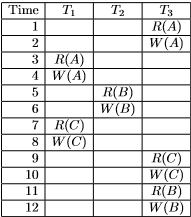
\includegraphics[width = 20em]{serializabilitySchedule1}
	\caption{Serializability Schedule, S1}
	\label{Serializability Schedule}
\end{figure}

\begin{enumerate}
	\item Is this schedule serial?
	\item  Give the dependency graph of this schedule.
	\item Is this schedule conflict serializable?
	\item  If you answer yes to the previous question, provide the equivalent serial schedule. If you answer no, briefly explain why.
	\item Could this schedule have been produced by 2PL?
\end{enumerate}

\paragraph{Answer 1}
	No, because transactions are strated before running transactions are completed. For instance transaction $T_2$ starts before $T_1$ has ended.
\pagebreak

\textbf{Answer 2}
\begin{figure}[H]
	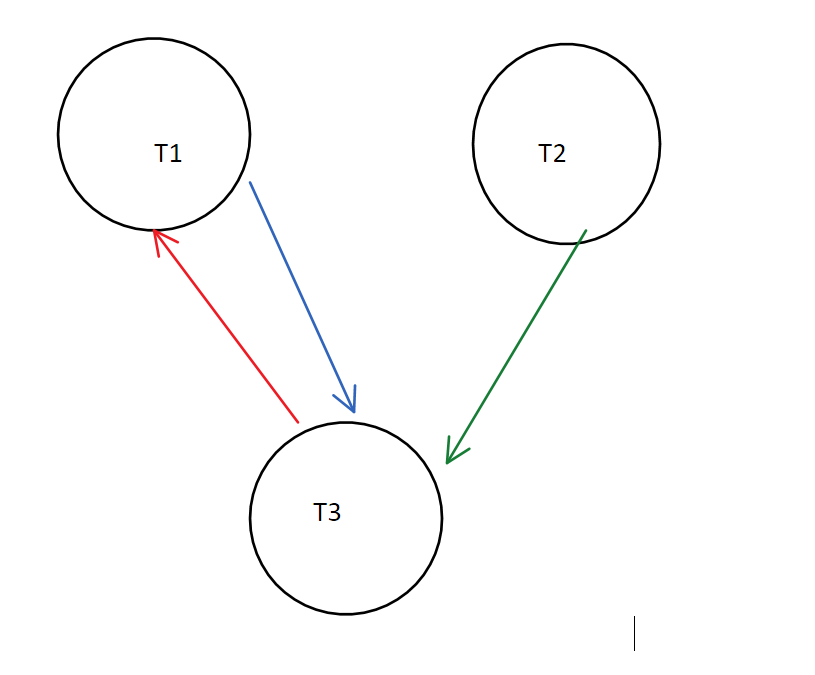
\includegraphics[width = 20em]{dependencyGraph}
	\label{Dependency Graph}
\end{figure}

\paragraph{Answer 3}
	No, because a schedule is conflict serializable if and only if the graph is acyclic. However, the graph contains a cycle between T1 and T3.
\paragraph{Answer 4}
	Not answered since no was stated in the answer above.
\paragraph{Answer 5}
	Yes it could have been produced by 2PL, because it is View Serializable. It is View Serializable because it is View Equivalent to the following schedule \textit{S2}:
	\begin{figure}[H]
	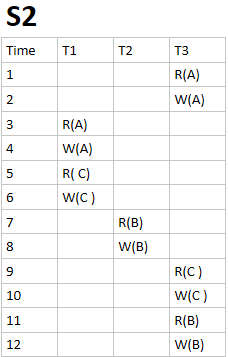
\includegraphics[width = 20em]{serializabilitySchedule2}
	\caption{Serializability Schedule, S2}
	\label{Serializability Schedule, S2}
\end{figure}
 and as such it upholds the 2PL Protocol's guarantee of serializability. 